\subsection{Autocorrelation Survey}
We performed the Ljung-Box test with the purpose of determining the presence of autocorrelation for the error term \(\varepsilon_t := \widehat{\text{RV}}_t - \text{RV}_t\). We present the results of the test in Table~\ref{tab:lijung_test}. We also present ACF and PACF plots in Figures~\ref{fig:har_acf+pacf} and~\ref{fig:garch_acf+pacf}.

\begin{table}[ht]
\centering
\begin{tabular}{|l|cc|cc|}
\hline
\textbf{Lag Number} & \multicolumn{2}{c|}{\textbf{HAR}} & \multicolumn{2}{c|}{\textbf{GARCH(1,1)}} \\
\textbf{} & \textbf{LB-Statistic} & \textbf{p-value} & \textbf{LB-Statistic} & \textbf{p-value} \\
\hline
\textbf{1} & 14.03 & 0.0 & 0.01 & 0.904228 \\
\hline
\textbf{2} & 20.61 & 0.000033 & 1.43 & 0.489933 \\
\hline
\textbf{3} & 22.28 & 0.000057 & 16.09 & 0.001089 \\
\hline
\textbf{4} & 22.28 & 0.000176 & 16.32 & 0.002619 \\
\hline
\textbf{5} & 23.84 & 0.000236 & 16.46 & 0.005656 \\
\hline
\end{tabular}
\caption{Statistical Tests Results for HAR and GARCH models}
\label{tab:lijung_test}

% HAR
%      lb_stat  lb_pvalue
% 1  14.026194   0.000180
% 2  20.610972   0.000033
% 3  22.275632   0.000057
% 4  22.282897   0.000176
% 5  23.814120   0.000236

% GARCH:
%     lb_stat  lb_pvalue
% 1   0.014477   0.904228
% 2   1.426972   0.489933
% 3  16.085860   0.001089
% 4  16.319778   0.002619
% 5  16.455883   0.005656



\end{table}


\begin{figure}[]
\centering
\begin{minipage}{.5\textwidth}
  \centering
  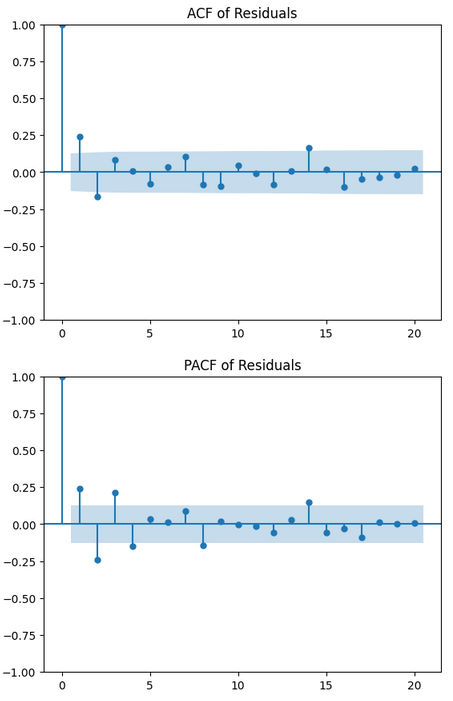
\includegraphics[width=.9\linewidth]{img/har_acf+pacf.png}
  \captionof{figure}{Plots for HAR residuals}
  \label{fig:har_acf+pacf}
\end{minipage}%
\begin{minipage}{.5\textwidth}
  \centering
  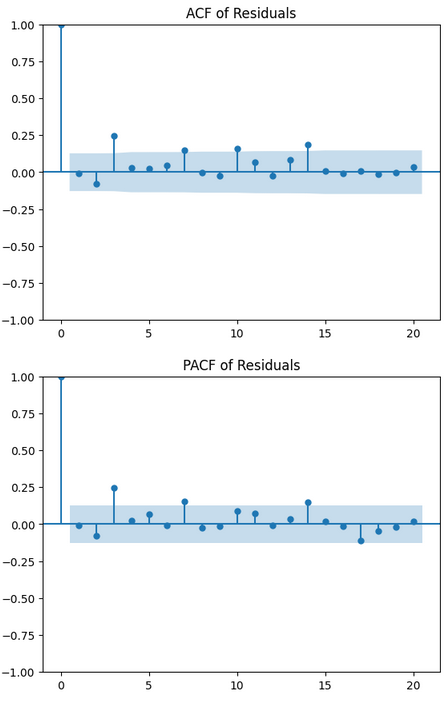
\includegraphics[width=.9\linewidth]{img/garch_acf+pacf.png}
  \captionof{figure}{Plots for GARCH residuals}
  \label{fig:garch_acf+pacf}
\end{minipage}
\end{figure}

As can be seen from these exhibits, strong autocorrelation exists in the residuals of the HAR model at all lags and in the residuals of the GARCH model at lags greater than 2. This potentially leaves room for improvement by creating a bagging-like model that utilizes an additional model (such as ARIMA or a more complex one) to predict the \(\varepsilon_t\) term.

\subsection{Bagging with ARIMA}

Both the HAR + ARIMA and GARCH + ARIMA combinations did not yield acceptable results because ARIMA could not successfully capture the underlying distribution of the \(\varepsilon_t\) term. This can be seen in Figure~\ref{fig:arima_fails}. Using a more sophisticated model instead of ARIMA seems like an interesting and promising experiment to the authors.

\begin{figure}
    \centering
    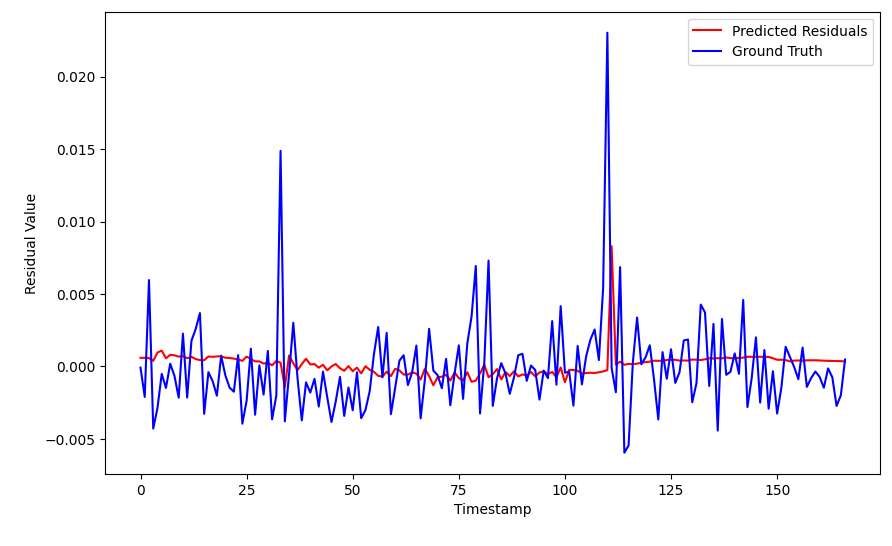
\includegraphics[width=0.9\linewidth]{img/arima_fails.png}
    \caption{ARIMA does not succeed in predicting the residual of RV}
    \label{fig:arima_fails}
\end{figure}

\subsection{Ensembling HAR and GARCH}
Due to the completely different nature of HAR and GARCH models, a natural idea emerges: combining their predictions into a new model. It was observed that the following estimates:
$$
\widehat{\text{RV}}_{\text{Ensemble}_1} := \alpha_1 \cdot \widehat{\text{RV}}_{\text{HAR}} + \alpha_2 \cdot \widehat{\text{RV}}_{\text{GARCH}}
$$
and 
$$
\widehat{\text{RV}}_{\text{Ensemble}_2} :=  \beta_1 \cdot \widehat{\text{RV}}_{\text{HAR}} + \beta_2 \cdot \widehat{\text{RV}}_{\text{GARCH}} + \beta_3 \cdot \widehat{\text{RV}}_{\text{Naive}}
$$
sometimes outperform all single-model predictions. However, one should be careful with tuning the \(\alpha\)'s. In our experiments, we chose \(\alpha_i := \frac{1}{2}\) and \(\beta_i := \frac{1}{3}\).

\subsection{Model Comparison}
In order to maintain readability, we present only a few examples of model evaluation metrics in Tables~\ref{tab:model_metrics_A} and~\ref{tab:model_metrics_B}. We also focused our attention on HAR-type models, since GARCH-based ones were already evaluated in previous work.

\vspace{10pt}

As can be seen from the Tables, both HAR and GARCH models typically outperform the naive volatility persistence model in our analysis. Among the various HAR specifications tested, the vanilla \textbf{HAR} and \textbf{HAR-J} models exhibited the best overall performance. However, it is important to note that the differences in performance among the various HAR and GARCH models were quite large, typically differing by up to 30\%. Notably, the GARCH model failed when predicting the ETH-USD data, but ensembles with GARCH performed competitively. In the case of BTC-USD data, Ensemble$_2$ significantly outperformed all other models.

\definecolor{neutral}{HTML}{CCCCCC}
\definecolor{green1}{HTML}{E6F9E6}  % Lightest green
\definecolor{green2}{HTML}{B8EB4A}  % Light green
\definecolor{green3}{HTML}{A6E22E}  % Medium green
\definecolor{green4}{HTML}{87D357}  % Slightly darker green
\definecolor{green5}{HTML}{6BBF2A}  % Darker green
\definecolor{green6}{HTML}{56A62A}  % Dark green
\definecolor{green7}{HTML}{3F8E23}  % Darker green
\definecolor{green8}{HTML}{2B7A1D}  % Even darker green
\definecolor{green9}{HTML}{1D6618}  % Very dark green
\definecolor{green10}{HTML}{0F5114} % Darkest green

\definecolor{yellow1}{HTML}{FFFFC5} % Light yellow

\begin{table}[ht]    
\begin{center}
    \begin{minipage}[t]{0.3\textwidth}
        \small % Reduce font size
        \caption{Performance Metrics for Model Evaluation on BTC-USD data}
        \label{tab:model_metrics_A}
        \sisetup{round-mode=places, round-precision=4, table-format=1.4}
        \begin{tabular}{l S[table-format=1.4] S[table-format=1.4]}
            \toprule
            \rowcolor{neutral!50} \textbf{Model} & \textbf{MSSE$^{-1}$} & \textbf{MAE$^{-1}$} \\
            \midrule
            Naive               & \cellcolor{green1}1.0000   & \cellcolor{green1}1.0000 \\
            HAR                 & \cellcolor{green3}1.1499   & \cellcolor{green3}1.1200 \\
            HAR-Q               & \cellcolor{green2}1.0029   & \cellcolor{green2}1.0382 \\
            HAR-J               & \cellcolor{green4}1.1298   & \cellcolor{green4}1.1124 \\
            GARCH               & \cellcolor{green2}1.0517   & \cellcolor{green2}1.0198 \\
            Ensemble$_1$           & \cellcolor{green5}1.1659   & \cellcolor{green5}1.1034 \\
            Ensemble$_2$       & \cellcolor{green6}1.3380   & \cellcolor{green6}1.1796 \\
            \bottomrule
        \end{tabular}
    \end{minipage}
    \hspace{50pt} % Adjust spacing if needed
    \begin{minipage}[t]{0.3\textwidth}
        \small % Reduce font size
        \caption{Performance Metrics for Model Evaluation on ETH-USD data}
        \label{tab:model_metrics_B}
        \sisetup{round-mode=places, round-precision=4, table-format=1.4}
        \begin{tabular}{l S[table-format=1.4] S[table-format=1.4]}
            \toprule
            \rowcolor{neutral!50} \textbf{Model} & \textbf{MSE$^{-1}$} & \textbf{MAE$^{-1}$} \\
            \midrule
            Naive               & \cellcolor{green1}1.0000   & \cellcolor{green1}1.0000 \\
            HAR                 & \cellcolor{green3}1.2038   & \cellcolor{green4}1.1445 \\
            HAR-Q               & \cellcolor{green3}1.1969   & \cellcolor{green3}1.1080 \\
            HAR-J               & \cellcolor{green4}1.2495   & \cellcolor{green5}1.1709 \\
            GARCH               & \cellcolor{yellow1}0.6564   & \cellcolor{yellow1}0.8563 \\
            Ensemble$_1$           & \cellcolor{green2}1.0233   & \cellcolor{green2}1.0248 \\
            Ensemble$_2$     & \cellcolor{green3}1.1947   & \cellcolor{green3}1.1083 \\
            \bottomrule
        \end{tabular}
    \end{minipage}
    \end{center}
\end{table}

